% !TEX root = ../mainthesis.tex

\chapter[Flexural strength and flaw distributions of \ce{SrFe_{0.2}Co_{0.4}Mo_{0.4}O_{3}} based ceramic-supports for solid-oxide fuel cells at operating conditions]{Flexural strength and flaw distributions of\\ \ce{SrFe_{0.2}Co_{0.4}Mo_{0.4}O_{3}} based ceramic-supports for \\solid-oxide fuel cells at operating conditions}

\section{Introduction}
    Most of the development focuses on the catalytic activity and conductivity enhancement in the material.
    However, an important characteristic of these materials that needs to be studied are the mechanical properties.
    An SOFC must be able to be adequately compressed to create a gas tight seal between the anode and cathode compartments for it to function well.
    This means that the cell must withstand the induced stresses from sealing, heating, and reduction by fuels.
    Redox cycling presents an additional challenge, especially in nickel-based systems, because oxidation and reduction phase changes cause crack growth and failure after a few cycles.\cite{Radovic2004, Radovic2004b, Laurencin2010, Pihlatie2009, Laurencin2009, Yu2007, Sarantaridis2007}
    A means of mitigating this problem is to use alternative, all ceramic anode system, such as \ce{La_{\hbox{1--x}}Sr_{x}Cr_{\hbox{1--y}}Mn_{y}O_{3}}, \ce{Sr_{0.94}Ti_{0.9}Nb_{0.1}O_{3-\delta}}, \ce{Ba_{0.98}La_{0.02}SnO_3}, or \ce{Sr_{2}MgMoO_{6}} (SMMO).\cite{Goodenough2007,Zha2005,Primdahl2001,Hussain2013,MohammedHussain2012,Hussain2016,Huang2006}

    One new material of interest is the double perovskite \ce{SrFe_{0.2}Co_{0.4}Mo_{0.4}O_{3}} (SFCM).\cite{Hussain,Hussaina,Pan}
    SFCM is a mixed ionic electronic conductor (MIEC) based off SMMO and other similarly structured anodes.
    The double perovskite family of materials, similar to SFCM and SMMO, have potential use as SOFC components due to the ability of the stable perovskite structure to generate and conduct oxygen vacancies and the multivalent cations allowing for electronic conduction and catalytic activity. \cite{Bernuy-Lopez2007, Huang2006a, Zhang2012}
    A similar thermal expansion of SFCM to GDC increases the compatibility between the components and reduces the chances of cracking and cell failure.
    SFCM has a high conductivity of \SI{\sim 35}{S\per\centi\meter} at \SI{650}{\celsius} and is stable to redox cycling making it a promising material.

    As an SOFC cell is heated and reduced, there is the possibility for changes to occur in the fracture toughness or flaw distribution of the materials.
    Heating causes the materials to expand, increasing their interatomic distances, and reduction creates oxygen vacancies weakening bonds.\cite{Boroomand2000,Bishop2009}
    Flaws can grow, combine, or change shape during these processes further affecting the overall strength.
    Equation \ref{eq:strength} demonstrates how various factors impact the strength of a sample, where $\sigma$ is the strength, $K_{Ic}$ is the fracture toughness, \textit{Y} is the shape factor for the flaw which caused failure and \textit{a} is the size of the flaw.\cite{Green1998}
    The fracture toughness and flaw distributions play a direct role in the overall strength of the cell.
    \begin{equation}
        \sigma = \frac{K_{Ic}}{Y\sqrt{a}}
        \label{eq:strength}
    \end{equation}

    Most research focuses on measuring and comparing the Young's moduli of different materials as it changes with environment.\cite{Gutierrez-Mora2002,Giraud2008,Kushi2011,Amezawa2011}
    While the modulus can be correlated to the fracture strength of the cell, direct measurement of flexural strength remains the best means to characterize the strength of the cell.
    This work characterizes the changes which occur in fracture toughness and flaw distributions of SFCM, SFCM-GDC anode support layer (ASL), and SFCM-GDC/GDC half-cells when exposed to oxidizing and reducing conditions up to \SI{600}{\celsius} by use of flexural testing and Weibull analysis.
    Additionally, electrical conductivity, thermogravimetric analysis, and thermal expansion are used to determine the causes for changes in mechanical properties under these conditions.

\section{Experimental}
    \subsection{Sample Preparation}
        SFCM powder was synthesized with conventional solid-state methods using stoichiometric amounts of strontium carbonate (\ce{SrCO_3}, Sigma-Aldrich), iron oxide (\ce{Fe_2O_3}, Sigma-Aldrich), cobalt oxide (\ce{Co_2O_3}, Inframat Advanced Materials), and molybdenum oxide (\ce{MoO_3}, Alfa-Aesar). The components were ball milled in ethanol for 24 hours, dried at \SI{100}{\celsius}, and heated to \SI{1100}{\celsius} for four hours.

        To create fracture toughness test samples, SFCM powder was ball milled overnight with a mixture of 0.6 wt\% polyethylene glycol 600, 1.8 wt\% ethylene glycol, and 0.6 wt\% glycerol in isopropyl alcohol.
        It was then dried at \SI{100}{\celsius}, ground by mortar and pestle, pressed uniaxially into rectangular bars at \SI{30}{\mega\pascal}, then isostatically pressed at \SI{30}{\mega\pascal}.
        Sintering followed by heating to \SI{1340}{\celsius} for four hours at \SI{3}{\celsius/min}  with a one hour hold at \SI{400}{\celsius} to allow the binders to burn out.
        This process achieved dense samples at 97\% average theoretical density with no apparent flaws in the bars.
        Bars were then cut and sanded to final dimensions of \SI{3}{mm} x \SI{4}{mm} x \SI{25}{mm}.
        The chevron notch was cut using the jig described by Jenkins, Chang and Okura following the ASTM procedure.\cite{Jenkins1988, ASTM2016a}

        Tape casting was used to create test coupons of porous SFCM-GDC ASL and half-cells.
        Using ethanol as a solvent, SFCM-GDC was ball milled with polyvinyl butyral, benzyl butyl phthalate, \SI{12}{\micro\meter} poly(methyl methacrylate) (16 wt\% with respect to SFCM-GDC), and Menhaden fish oil.
        The tape was cast to a thickness of \SI{110}{\micro\meter} on Mylar then laminated using a hot press to a final thickness of \SI{660}{\micro\meter}.
        Dense GDC was casted to \SI{30}{\micro\meter} and laminated to the top of the SFCM-GDC to create half-cells.
        Individual coupons were cut from the green tape, sintered at \SI{1200}{\celsius} for four hours, with holds at low temperatures to burn out organic binder and pore former.
        The final thicknesses were measured to be \SI{400}{\micro\meter} for the SFCM-GDC ASL and \SI{\sim 20}{\micro\meter} thick GDC electrolyte.
        Test coupons had their edges sanded to remove defects left from cutting, following ASTM standards.\cite{ASTM2008}
        Top and bottom surfaces were not sanded to preserve possible defects left from tape casting procedure, which would be representative of industrially manufactured SOFCs.

        X-ray diffraction (XRD) was used to check and confirm phase purity of SFCM samples throughout the preparation and testing process.
        A Bruker D8 Advance with LynxEye was used with a Cu K\textsubscript{\textalpha{}} source.
        A step size of \SI{0.02}{\degree} was used with a dwell of \SI{0.8}{\second} to obtain diffraction patterns.

    \subsection{Conductivity}
        Direct current conductivity was measured using rectangular bars of SFCM and SFCM-GDC (2:1) composite.
        The samples were connected to a Keithley 2400 source meter by silver paste and wire.
        Using an in-house built reactor, the sample could be heated and the gas environment could be controlled.
        An initial measurement was taken after heating and 50 hours of exposure to 10\% H\textsubscript{2} in N\textsubscript{2}, then the sample exposed cycled between air and reducing conditions over a period of 14 days.

    \subsection{Thermogravimetric Analysis (TGA)}
        Mass of samples during oxidation and reduction cycling was measured using a Cahn D200 microbalance.
        The samples were placed in a crucible suspended from a platinum wire attached to the microbalance and enclosed by an alumina tube inside a furnace.
        Heating control was achieved with a PID loop and temperature measurement done by a K-type thermocouple placed immediately below the sample inside the alumina tube.
        Gas flow was controlled at a constant \SI{50}{sccm} by mass flow controllers.
        21\% O\textsubscript{2} in dry N\textsubscript{2} was used for the oxidizing condition while 3\% H\textsubscript{2} in N\textsubscript{2} humidified with 3\% H\textsubscript{2}O was used for the reducing conditions.

    \subsection{Mechanical Measurements}
        Measurements of mechanical properties were collected using a Tinius Olsen 10ST Universal Testing Machine equipped with a \SI{250}{N} load cell.
        Experiments where any samples would be tested at elevated temperatures or under reducing environments were conducted using a custom built three point flexural test fixture placed inside a gas-tight chamber and furnace.
        Otherwise, a fully-articulating four point flexural test fixture was used.
        Samples tested at ambient conditions were placed on the appropriate testing fixture and loaded until failure.
        For samples tested at elevated temperatures the sample was heated in the test chamber at \SI{10}{\celsius\per\minute}, allowed to equilibrate for 20 minutes, then tested.
        Samples to be reduced were placed in the chamber, heated and exposed to reducing gas for 18 hours before being tested.

    \subsubsection{Flexural Strength}
        A loading rate of \SI{0.2}{mm\per\minute} was used for all strength measurements.
        Strength was calculated from the maximum force measured before failure according to Equation \ref{eq:4ptstrength} or \ref{eq:3ptstrength} depending on if the four point or three point fixture is used respectively, where $\sigma{}$ is the strength, \textit{P} is the maximum force, \textit{L} is the span width of the test fixture, \textit{b} is the width of the sample and \textit{d} is the thickness of the sample. Equation \ref{eq:4ptstrength} is for a fixture where the top span is 1/2 the width of the bottom span.\cite{ASTM2008}
        \begin{equation}
            \sigma = \frac{3PL}{4bd^{2}}
            \label{eq:4ptstrength}
        \end{equation}

    \subsubsection{Chevron Notch Fracture Toughness}
        The fracture toughness of chevron notched samples were measured using a loading rate of \SI{0.001}{mm\per\minute}.
        Fracture toughness was calculated from the maximum force using Equation \ref{eq:4ptkivb} or \ref{eq:3ptkivb} for four point or three point fixtures.\cite{ASTM2016a,Wu1984}
        $Y^{*}_{min}$ is the shape factor as calculated by Equation \ref{eq:shapefactor}, $S_o$ and $S_i$ are the outer and inner spans, \textit{B} is the width of the sample, \textit{W} is the height of the sample, $a_0$ is the distance from the tip of the chevron notch to the bottom of the sample, and $a_1$ is the average distance from the side of the chevron notch to the bottom of the sample.
        Each sample was measured after failure, but in this study the approximate values were $S_o = 40 mm$, $S_i = 20 mm$, $B = 3.0 mm$, $W = 4.0 mm$, $a_0 = 0.80 mm$, $a_1 = 3.8 mm$.
        Fracture toughness was measured only under air at room temperature and up to \SI{600}{\celsius}.
        Under reduction the fracture toughness bars would spontaneously fracture, preventing measurements under that condition.
        \begin{equation}
            K_{Ivb} = Y^{*}_{min}  \left [\frac{P[S_o-S_i]}{BW^{3/2}}\right ]10^{-6}
            \label{eq:4ptkivb}
        \end{equation}
        \begin{equation}
            K_{Ivb} = Y^{*}_{min}  \left [\frac{P}{BW^{1/2}}\right ]10^{-6}
            \label{eq:3ptkivb}
        \end{equation}
        \begin{equation}
            Y^{*}_{min} = \frac{0.38742-3.0919(a_0/W)+4.2017(a_1/W)-2.3127(a_1/W)^2+0.6379(a_1/W)^3}{1.0000-2.9686(a_0/W)+3.5056(a_0/W)^2-2.1374(a_0/W)^3+0.0130(a_1/W)}
            \label{eq:shapefactor}
        \end{equation}

\section{Results and Discussion}
    \subsection{Redox Cycling Stability}
        SFCM has a high initial conductivity of \SI{35}{S\per\centi\meter} but decreases after 3 cycles to \SI{19}{S\per\centi\meter} and again at 9 cycles, shown in Figure \ref{fig:TGA}a.
        The addition of GDC to create a SFCM-GDC composite decreases the initial conductivity to \SI{15}{S\per\centi\meter}.
        At 4 cycles, SFCM-GDC decreases conductivity and stabilizes to \SI{8}{S\per\centi\meter} for 19 cycles.
        The addition of the GDC improved the redox cycling stability by providing a very stable, contiguous framework for the SFCM.\cite{Mogensen2000,Duncan2006,Bishop2009}

        Figure \ref{fig:TGA}b shows the mass loss of SFCM-GDC as it is reduced in 3\% humidified H\textsubscript{2}.
        For comparison, another popular anode material, nickel oxide GDC, is plotted along with it.
        The reduction of SFCM-GDC results in a less than 1\% reduction of mass from the formation of oxygen vacancies in the SFCM and GDC, and it reaches steady state in under two hours.
        NiO-GDC on the other hand loses a large amount of mass from the reduction and phase change of NiO to Ni metal taking over 30 hours to reach steady state.

        \begin{figure}
          \includegraphics[width=0.45\textwidth]{CycleConductivity.jpg}
          \includegraphics[width=0.45\textwidth]{TGA.jpg}
          \caption{a) DC conductivity of SFCM and SFCM-GDC after cycling at \SI{650}{\celsius} between 10\% H\textsubscript{2} in N\textsubscript{2} and air. b) Mass loss of SFCM-GDC and NiO-GDC during reduction in 3\% H\textsubscript{2}/3\% H\textsubscript{2}O in N\textsubscript{2} at \SI{650}{\celsius}.}
          \label{fig:TGA}
        \end{figure}

        Further cycling of SFCM in the thermogravimetric analyzer (TGA) was performed and results are given in Figure \ref{fig:Cycled} with \ref{fig:Cycled}a showing the mass loss of SFCM with time as it is cycled between air and hydrogen and \ref{fig:Cycled}b being a summary of the total mass changes that occur with each cycle.
        With each cycle, less than 1\% total mass change is observed.
        Reduction occurs over a time period of five hours while oxidation happens at a faster rate, approximately one hour.
        Fitting the reduction and oxidation to exponential functions gives a biexponential with decay rates of 0.438 and 27.89 for reduction and an oxidation rate of 2.90.
        This demonstrates that SFCM does not generate any additional phases which cause the loss or gain of oxygen and that reduction and oxidation are reversible processes which occur over short periods.

        \begin{figure}
          \includegraphics[width=0.45\textwidth]{TGACycle.jpg}
          \includegraphics[width=0.45\textwidth]{CycleSummary.jpg}
          \caption{Mass changes of SFCM during cycling between 21\% O\textsubscript{2} and 3\% H\textsubscript{2}/3\% H\textsubscript{2}O in N\textsubscript{2} at \SI{600}{\celsius}. Each exposure was 5 hours. a) Percent mass change with time as the gas is switched back and forth. b) Summary of maximum and minimum changes with each cycle.}
          \label{fig:Cycled}
        \end{figure}

    \subsection{Fracture Toughness}
        Fracture toughness was found to be \SI[separate-uncertainty = true]{0.124 +- 0.023}{\mega\pascal\sqrt{m}} at room temperature, increasing with temperature up to \SI{600}{\celsius}, as shown in Figure \ref{fig:Kic}a.
        From room temperature to \SI{500}{\celsius}, the rate of increase in K\textsubscript{Ic} is low at \SI{4.3e-5}{\mega\pascal\sqrt{m}\per\celsius}.
        From \SI{500}{\celsius} to \SI{600}{\celsius} the fracture toughness increases by 90\%.
        The increase in fracture toughness is a result of the thermal expansion of the material.
        During process of creating the bar, the sample was cooled from \SI{1340}{\celsius} to room temperature.
        This cooling and associated contraction induces stresses in the bar sample, which combine with the stresses added during testing to fracture the sample.
        As the sample is heated, the residual stresses are relaxed, increasing the amount of stress which must be applied externally to cause the bar to fracture.
        Any change in fracture toughness due to the weakening of bonds is masked by this effect.
        The increase in fracture toughness from \SI{500}{\celsius} to \SI{600}{\celsius} matches the temperature where the rate of thermal expansion also increases, as shown in Figure \ref{fig:Kic}b.

        Figure \ref{fig:Kic}b also presents the thermal expansion of GDC and a SFCM-GDC composite.
        At temperatures below \SI{550}{\celsius} the expansion of SFCM-GDC matches that of pure SFCM, greater than that of pure GDC.
        Above \SI{550}{\celsius}, the rate of expansion slows in comparison to SFCM and matches the rate of expansion for GDC.
        Thus, below \SI{550}{\celsius}, SFCM-GDC expands the same as SFCM and above \SI{550}{\celsius} it expands the same as GDC.
        We would then expect that SFCM-GDC composites have the same increase in fracture toughness as SFCM up to \SI{550}{\celsius} due expansion and relaxation of intrinsic stresses, but not further increase the rate above \SI{500}{\celsius}, as SFCM does.

        \begin{figure}
            \includegraphics[width=0.45\textwidth]{Kic.jpg}
            \includegraphics[width=0.45\textwidth]{ThermalExpansion.jpg}
            \caption{a) Fracture toughness of SFCM from \SI{20}{\celsius} to \SI{600}{\celsius}. b) Thermal expansion of SFCM, GDC, and SFCM-GDC.}
            \label{fig:Kic}
        \end{figure}

    \subsection{Half-cell Strength of Anode-Supported SOFCs at Operating Conditions}
        Figure \ref{fig:InSituBox} gives box plots of the results of three point flexural testing of SFCM-GDC/GDC half-cells, and Table \ref{tab:halfcell} summaries the strengths.
        The circles on the right of \ref{fig:InSituBox} represent the results of a Student's t-test, to determine if the means of the different data sets are the same.
        The more the circles overlap the more similar the data sets are.
        In this case, there is no overlap between circles at the 95\% confidence interval, highlighting that the strengths tested at each condition are unique from each other.

        At ambient conditions the strength of the half-cells was measured to be \SI{57.7}{\mega\pascal}.
        Upon heating, the strength increases to \SI{74.2}{\mega\pascal}.
        This result correlates with the increase in fracture toughness discussed earlier, which is expected based on Equation \ref{eq:strength}.
        Another contributing factor to the increase in strength is the effect thermal expansion has on pre-existing cracks and flaws.
        Any expansion of the material helps push closed a surface crack which would lead to failure, decreasing its size and increasing the stress that would be required to cause that crack to open and propagate.

        Upon reduction of the half-cell at \SI{600}{\celsius}, the fracture strength decreases, below that of the ambient strength, to \SI{39.9}{\mega\pascal}.
        This reduction of strength is likely due to the combination of the decrease in fracture toughness and the growth of microcracks as the materials reduce in volume.

        \begin{figure}
          \includegraphics[width=\textwidth]{halfcellstrength.png}
          \caption{Flexural strengths of half-cell coupons made from SFCM-GDC anode with GDC electrolyte tested at \SI{20}{\celsius} in air, \SI{600}{\celsius} in air, and \SI{600}{\celsius} in 5\% H\textsubscript{2}.}
          \label{fig:InSituBox}
        \end{figure}

        \begin{table}
            \centering
            \caption{Summary of strengths for SFCM-GDC/GDC half-cells at different environments}
            \label{tab:halfcell}
            \begin{tabular}{lllll}
            \begin{tabular}[c]{@{}l@{}}Temperature\\(\SI{}{\celsius})\end{tabular} & Atmosphere & Number & \begin{tabular}[c]{@{}l@{}}Mean\\(MPa)\end{tabular} & \begin{tabular}[c]{@{}l@{}}Std Dev\\(MPa)\end{tabular}  \\
            \hline
            20                                                       & Air        & 17      & 57.7                                                & 6.71                                                    \\
            600                                                      & Air        & 5      & 74.2                                                & 2.98                                                    \\
            600                                                      & 5\% H2     & 14      & 39.9                                                & 5.89
            \end{tabular}
        \end{table}

        Weibull analysis was performed to compare the distribution of flaws between the ambient tested half-cells and the in-situ reduced half-cells.
        Figure \ref{fig:halfcellweibull} displays the fitting of Weibull distributions to the flexural strength of half-cell coupons tested at ambient conditions and during reduction at \SI{600}{\celsius}.
        Table \ref{tab:InSituWeibull} summarizes the fitting parameter for the Weibull modulus with 95\% confidence intervals using the maximum-likelihood method.
        Between the two conditions, there is an appreciable change in the Weibull modulus of the two samples.
        The Weibull modulus increases decreases from 10.4 at ambient conditions to 7.29 when at reducing conditions.
        This indicates that the distribution of flaws has changed by becoming wider, creating more variability between flaws.
        It is possible that this change is the result of an uneven growth of two different flaw types.

        To confirm this, fractography would need to be performed on every sample, identifying the flaw, but this is not possible due to the porous nature of the fracture surface which obscures the fracture origin.
        Scanning electron microscopy was performed on fracture surfaces and epoxy filled  samples from each condition to look for any microstructural changes.
        Figure \ref{fig:InSituSEM} shows the epoxy filled and polished samples with no discernible difference between samples.
        No difference is observed because the likely cause of failure, microcracks, would exist along grain boundaries and are obscured by the grain boundaries and pores.\cite{Danzer2008,Yu2007}

        \begin{figure}
          \includegraphics[width=0.8\textwidth]{insituweibull.png}
          \caption{Fitted Weibull distributions of SFCM-GDC/GDC half-cells at different environments, plotted linearly with 95\% confidence intervals shaded.}
          \label{fig:halfcellweibull}
        \end{figure}

        \begin{table}
            \centering
            \caption{Summary of Weibull fitting parameters (characteristic strength and Weibull modulus) for SFCM-GDC/GDC half-cells at different environments}
            \label{tab:InSituWeibull}
            \begin{tabular}{llrrrrrr}
            \begin{tabular}[c]{@{}l@{}}Temp.~\\(\SI{}{\celsius})\end{tabular} & Environment & \multicolumn{1}{l}{\begin{tabular}[c]{@{}l@{}}Cha.~\\Strength\\(\textalpha{}, \SI{}{\mega\pascal})\end{tabular}} & \multicolumn{1}{l}{\begin{tabular}[c]{@{}l@{}}\textalpha~\\Lower\\CI\end{tabular}}& \multicolumn{1}{l}{\begin{tabular}[c]{@{}l@{}}\textalpha~\\Upper\\CI\end{tabular}}& \multicolumn{1}{l}{\begin{tabular}[c]{@{}l@{}}Weibull~\\Modulus\\ (\textbeta)\end{tabular}}& \multicolumn{1}{l}{\begin{tabular}[c]{@{}l@{}}\textbeta~\\Lower\\CI\end{tabular}}& \multicolumn{1}{l}{\begin{tabular}[c]{@{}l@{}}\textbeta~\\Upper\\CI\end{tabular}}  \\
            \hline
            20                                                        & Air         & 60.6                                                                                           & 57.4& 63.6& 10.4& 6.89& 14.7                                                                              \\
            600                                                       & Hydrogen    & 42.5                                                                                           & 39.2& 45.8& 7.29& 4.79& 10.3
            \end{tabular}
        \end{table}

        \begin{figure}
          \includegraphics[width=0.45\textwidth]{RTFracture.jpg}
          \includegraphics[width=0.45\textwidth]{HTfracture.jpg}
          \includegraphics[width=0.45\textwidth]{ReduceFracture.jpg}
          \caption{Scanning electron microscope images of epoxy filled and polished SFCM-GDC/GDC half-cell cross sections tested at a) \SI{20}{\celsius} in air, b) \SI{600}{\celsius} in air and c)\SI{600}{\celsius} in 5\% H\textsubscript{2}.}
          \label{fig:InSituSEM}
        \end{figure}

    \subsection{Strength of Anode Support Layer After Redox Cycling}
        To understand how redox cycling as the result of long term use affects the strength of SFCM based SOFCs, SFCM-GDC ASL test coupons were cycled for 10 times between nitrogen and 10\% H\textsubscript{2} environments.
        Figure \ref{fig:cycledbox} shows the strength and modulus from the samples which were not cycled (0 cycles) and those cycled 10 times, tested using a four-point bend at ambient conditions.
        Table \ref{tab:cycledsummary} summaries the means and standard deviations of the test results.
        The overlapping Student's t circles in Figure \ref{fig:cycledbox}b demonstrate that cycling did not significantly change the elastic modulus of the samples, while the strength did significantly decrease.
        This is the result of changes in microstructural flaws, rather than the change of an intrinsic material property.

        \begin{figure}
          \includegraphics[width=5in]{cycledbox.png}
          \includegraphics[width=5in]{cycledmod.png}
          \caption{Results of four point bend test at ambient conditions of SFCM-GDC ASL with a) strength and b) modulus for samples before any cycling and after 10 redox cycles between 10\% H\textsubscript{2} and N\textsubscript{2}.}
          \label{fig:cycledbox}
        \end{figure}

        \begin{table}
            \centering
            \caption{Summary of Cycled SFCM-GDC ASL Mechanical Properties}
            \label{tab:cycledsummary}
            \begin{tabular}{llllll}
            \begin{tabular}[c]{@{}l@{}}Number~\\of Cycles\end{tabular} & Number &  \begin{tabular}[c]{@{}l@{}}Mean~\\Modulus~\\(GPa)\end{tabular}& \begin{tabular}[c]{@{}l@{}}Modulus\\Std Dev~\\(GPa)\end{tabular}& \begin{tabular}[c]{@{}l@{}}Mean\\Strength\\(MPa)\end{tabular} & \begin{tabular}[c]{@{}l@{}}Strength~\\Std Dev~\\(MPa)\end{tabular} \\
            \hline
            0                                                          & 14     & 24.5                                                          & 5.01& 34.3& 7.23                                                                                                                                                                                      \\
            10                                                         & 20     & 27.3                                                          & 3.60& 22.4& 4.94
            \end{tabular}
        \end{table}

        The strengths of the cycled and un-cycled cells were fitted to Weibull distributions to observe how flaw distributions changed with redox cycling.
        Figure \ref{fig:cycledweibull} presents the fitted data and distributions and Table \ref{tab:cycledweibull} summarizes the fit parameters of the Weibull modulus with 95\% confidence intervals.
        The Weibull moduli between the two data sets are very similar, indicating that the flaw distribution is the same between them.
        The decrease in characteristic strength is then due to the growth of flaws with cycling.
        SEM images in Figure \ref{fig:cycledSEM} are of a sample which had not been cycled (a) and one which had been cycled 10 times (b) after being epoxy filled and polished.
        The sample which had been cycled 10 times has a greater number of pores at larger sizes compared to the un-cycled sample.
        This indicates that the finer microstructure of the pores is susceptible to changes during redox cycling due to chemical expansion, but the larger flaws which lead to complete cell failure do not change as the result of redox cycling.\cite{Waldbillig2005}

        \begin{figure}
          \includegraphics[width=4in]{cycledweibull.png}
          \caption{Fitted Weibull distributions of SFCM-GDC ASL before any cycling and after 10 redox cycles between 10\% H\textsubscript{2} and N\textsubscript{2}, plotted linearly with 95\% confidence intervals shaded}
          \label{fig:cycledweibull}
        \end{figure}

        \begin{table}
        \centering
        \caption{Summary of Weibull Fit Parameters (characteristic strength and Weibull modulus) for Cycled SFCM-GDC ASL}
        \label{tab:cycledweibull}
        \begin{tabular}{lrrrrrr}
        \begin{tabular}[c]{@{}l@{}}Number\\of Cycles\end{tabular} & \multicolumn{1}{l}{\begin{tabular}[c]{@{}l@{}}Char.~\\Strength~\\(\textalpha{}, \SI{}{\mega\pascal})\end{tabular}} & \multicolumn{1}{l}{\begin{tabular}[c]{@{}l@{}}\textalpha{}~\\CI Lower\end{tabular}} & \multicolumn{1}{l}{\begin{tabular}[c]{@{}l@{}}\textalpha{}~\\CI Upper\end{tabular}}& \multicolumn{1}{l}{\begin{tabular}[c]{@{}l@{}}Weibull~\\Modulus~\\(\textbeta{})\end{tabular}}& \multicolumn{1}{l}{\begin{tabular}[c]{@{}l@{}}\textbeta{}~\\CI Lower\end{tabular}}& \multicolumn{1}{l}{\begin{tabular}[c]{@{}l@{}}\textbeta{}~\\CI Upper\end{tabular}}  \\
        \hline
        0                                                         & 37.1                                                                                    & 33.7                                                                     & 40.8& 5.75& 4.06& 9.85                                                                                   \\
        10                                                        & 24.3                                                                                    & 22.3                                                                     & 26.5& 5.39& 4.00& 8.28
        \end{tabular}
        \end{table}

        \begin{figure}
          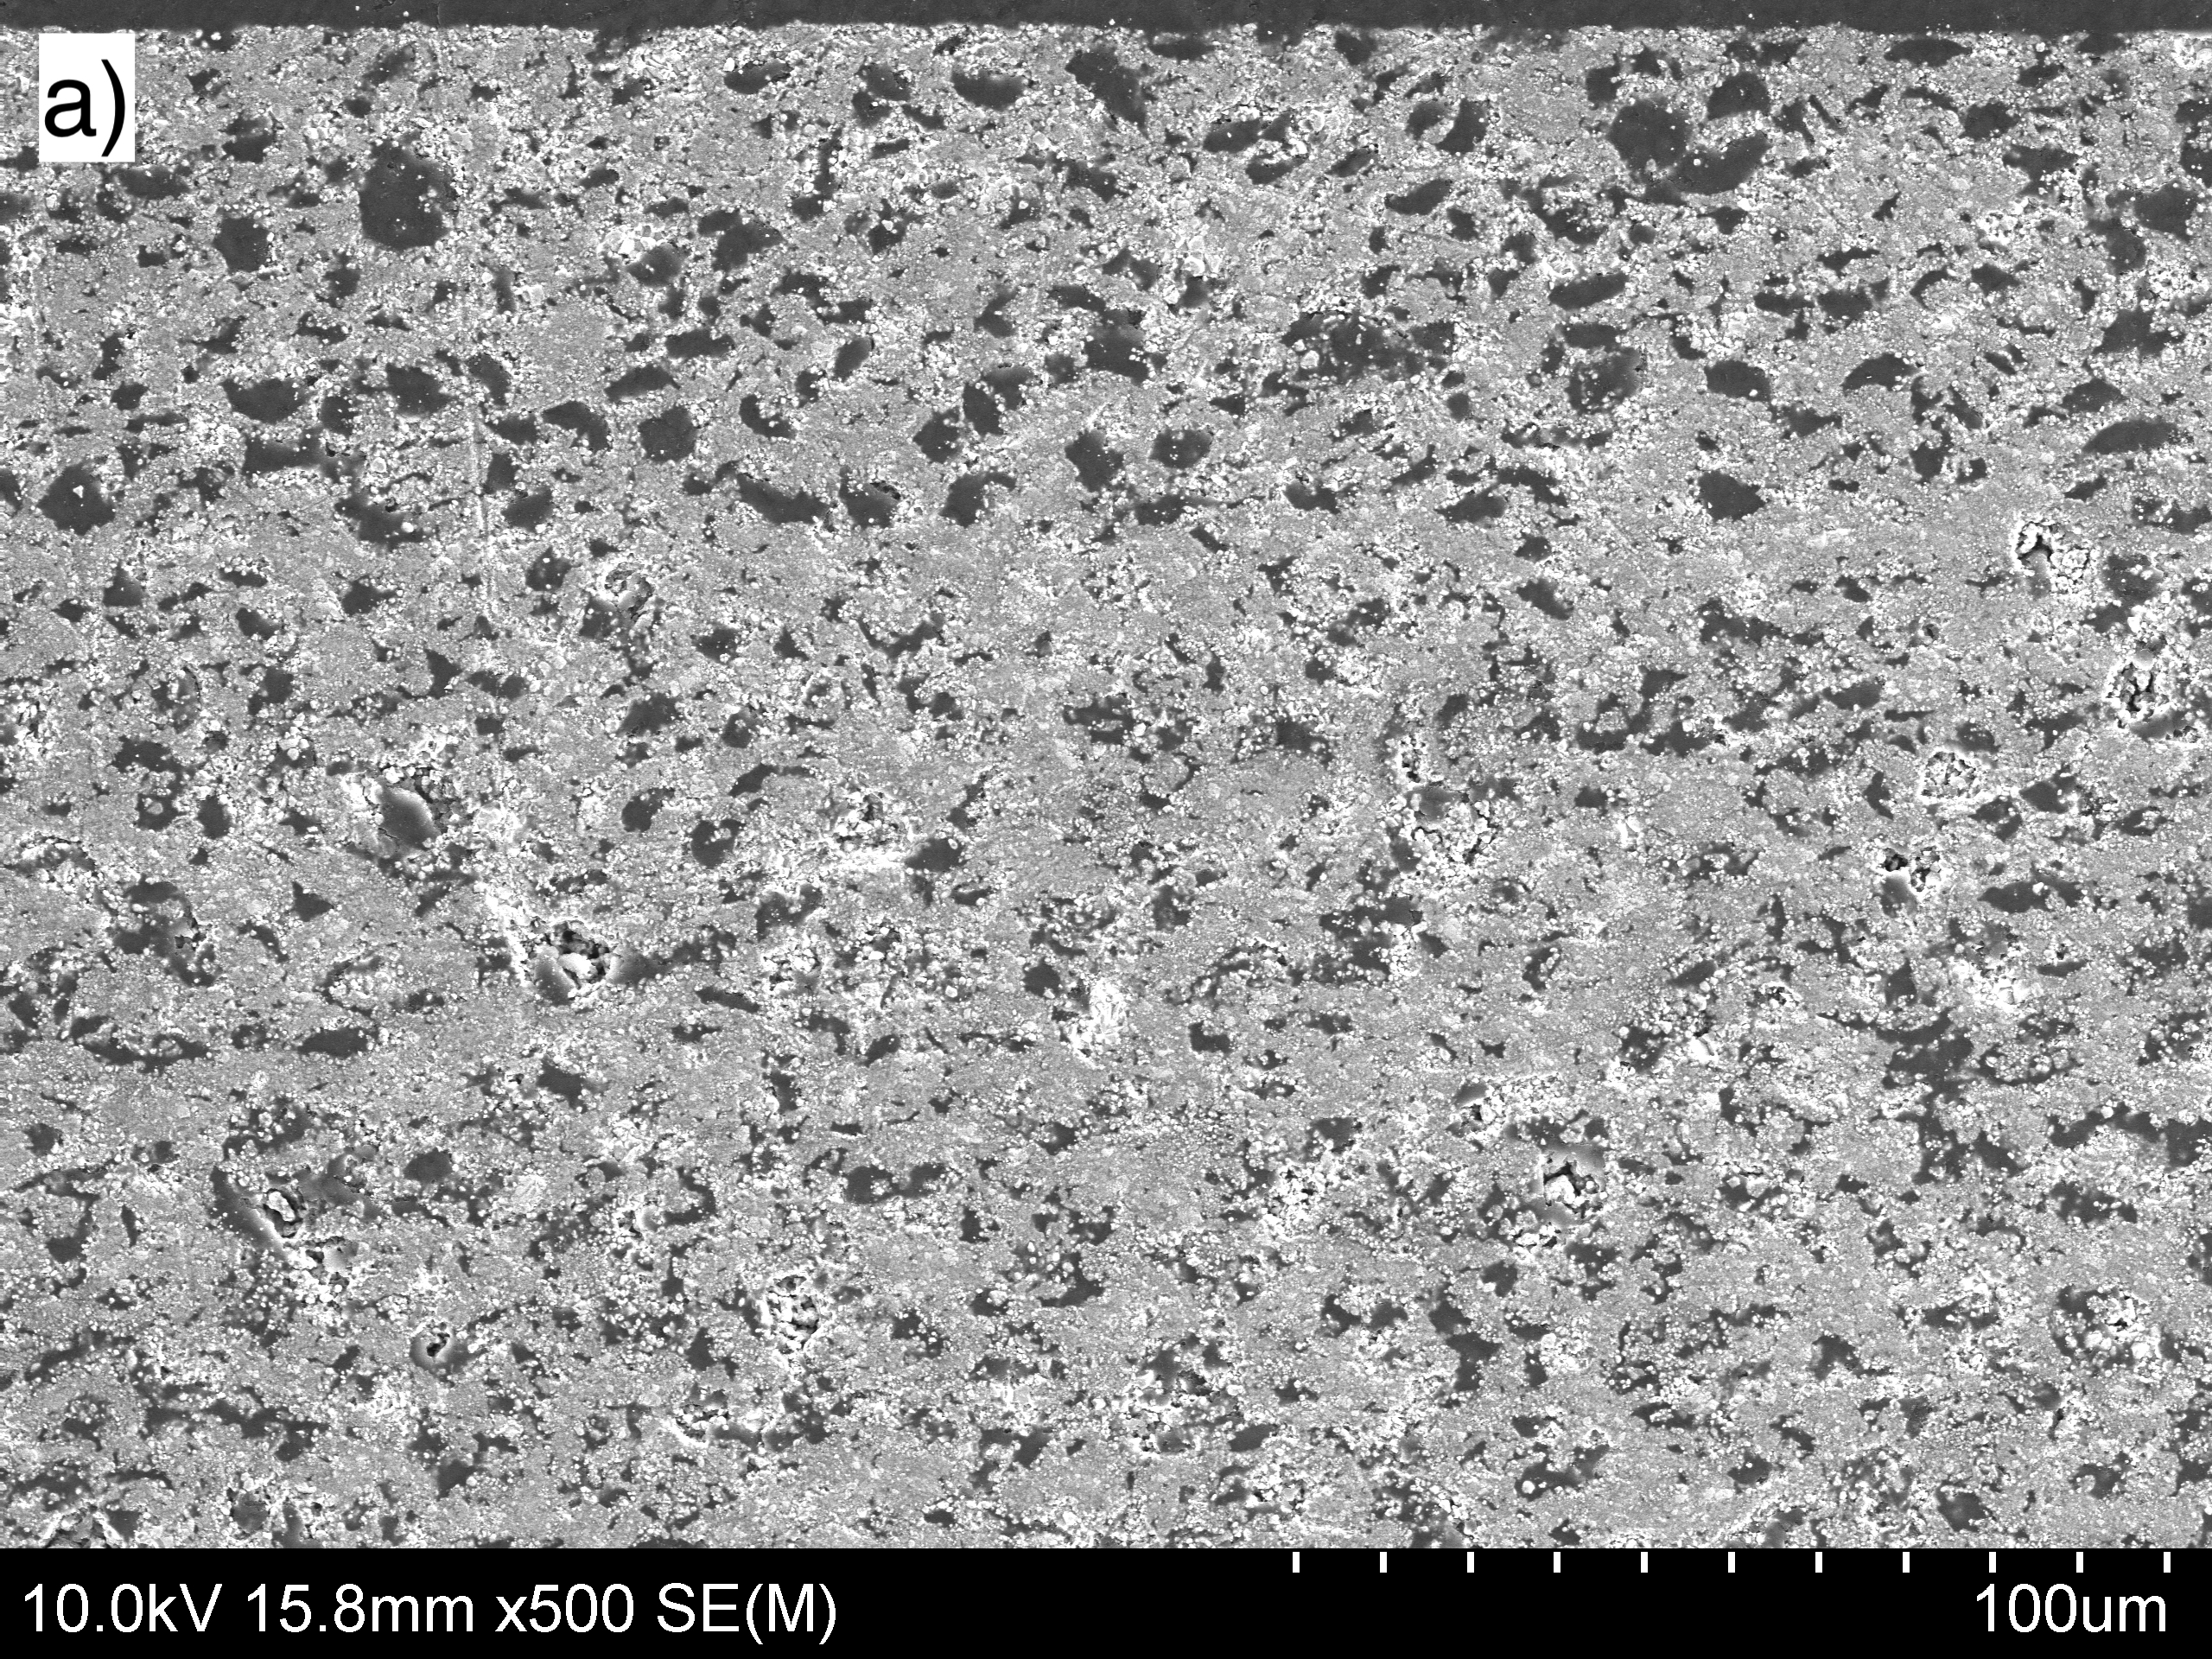
\includegraphics[width=0.45\textwidth]{0cycles.jpg}
          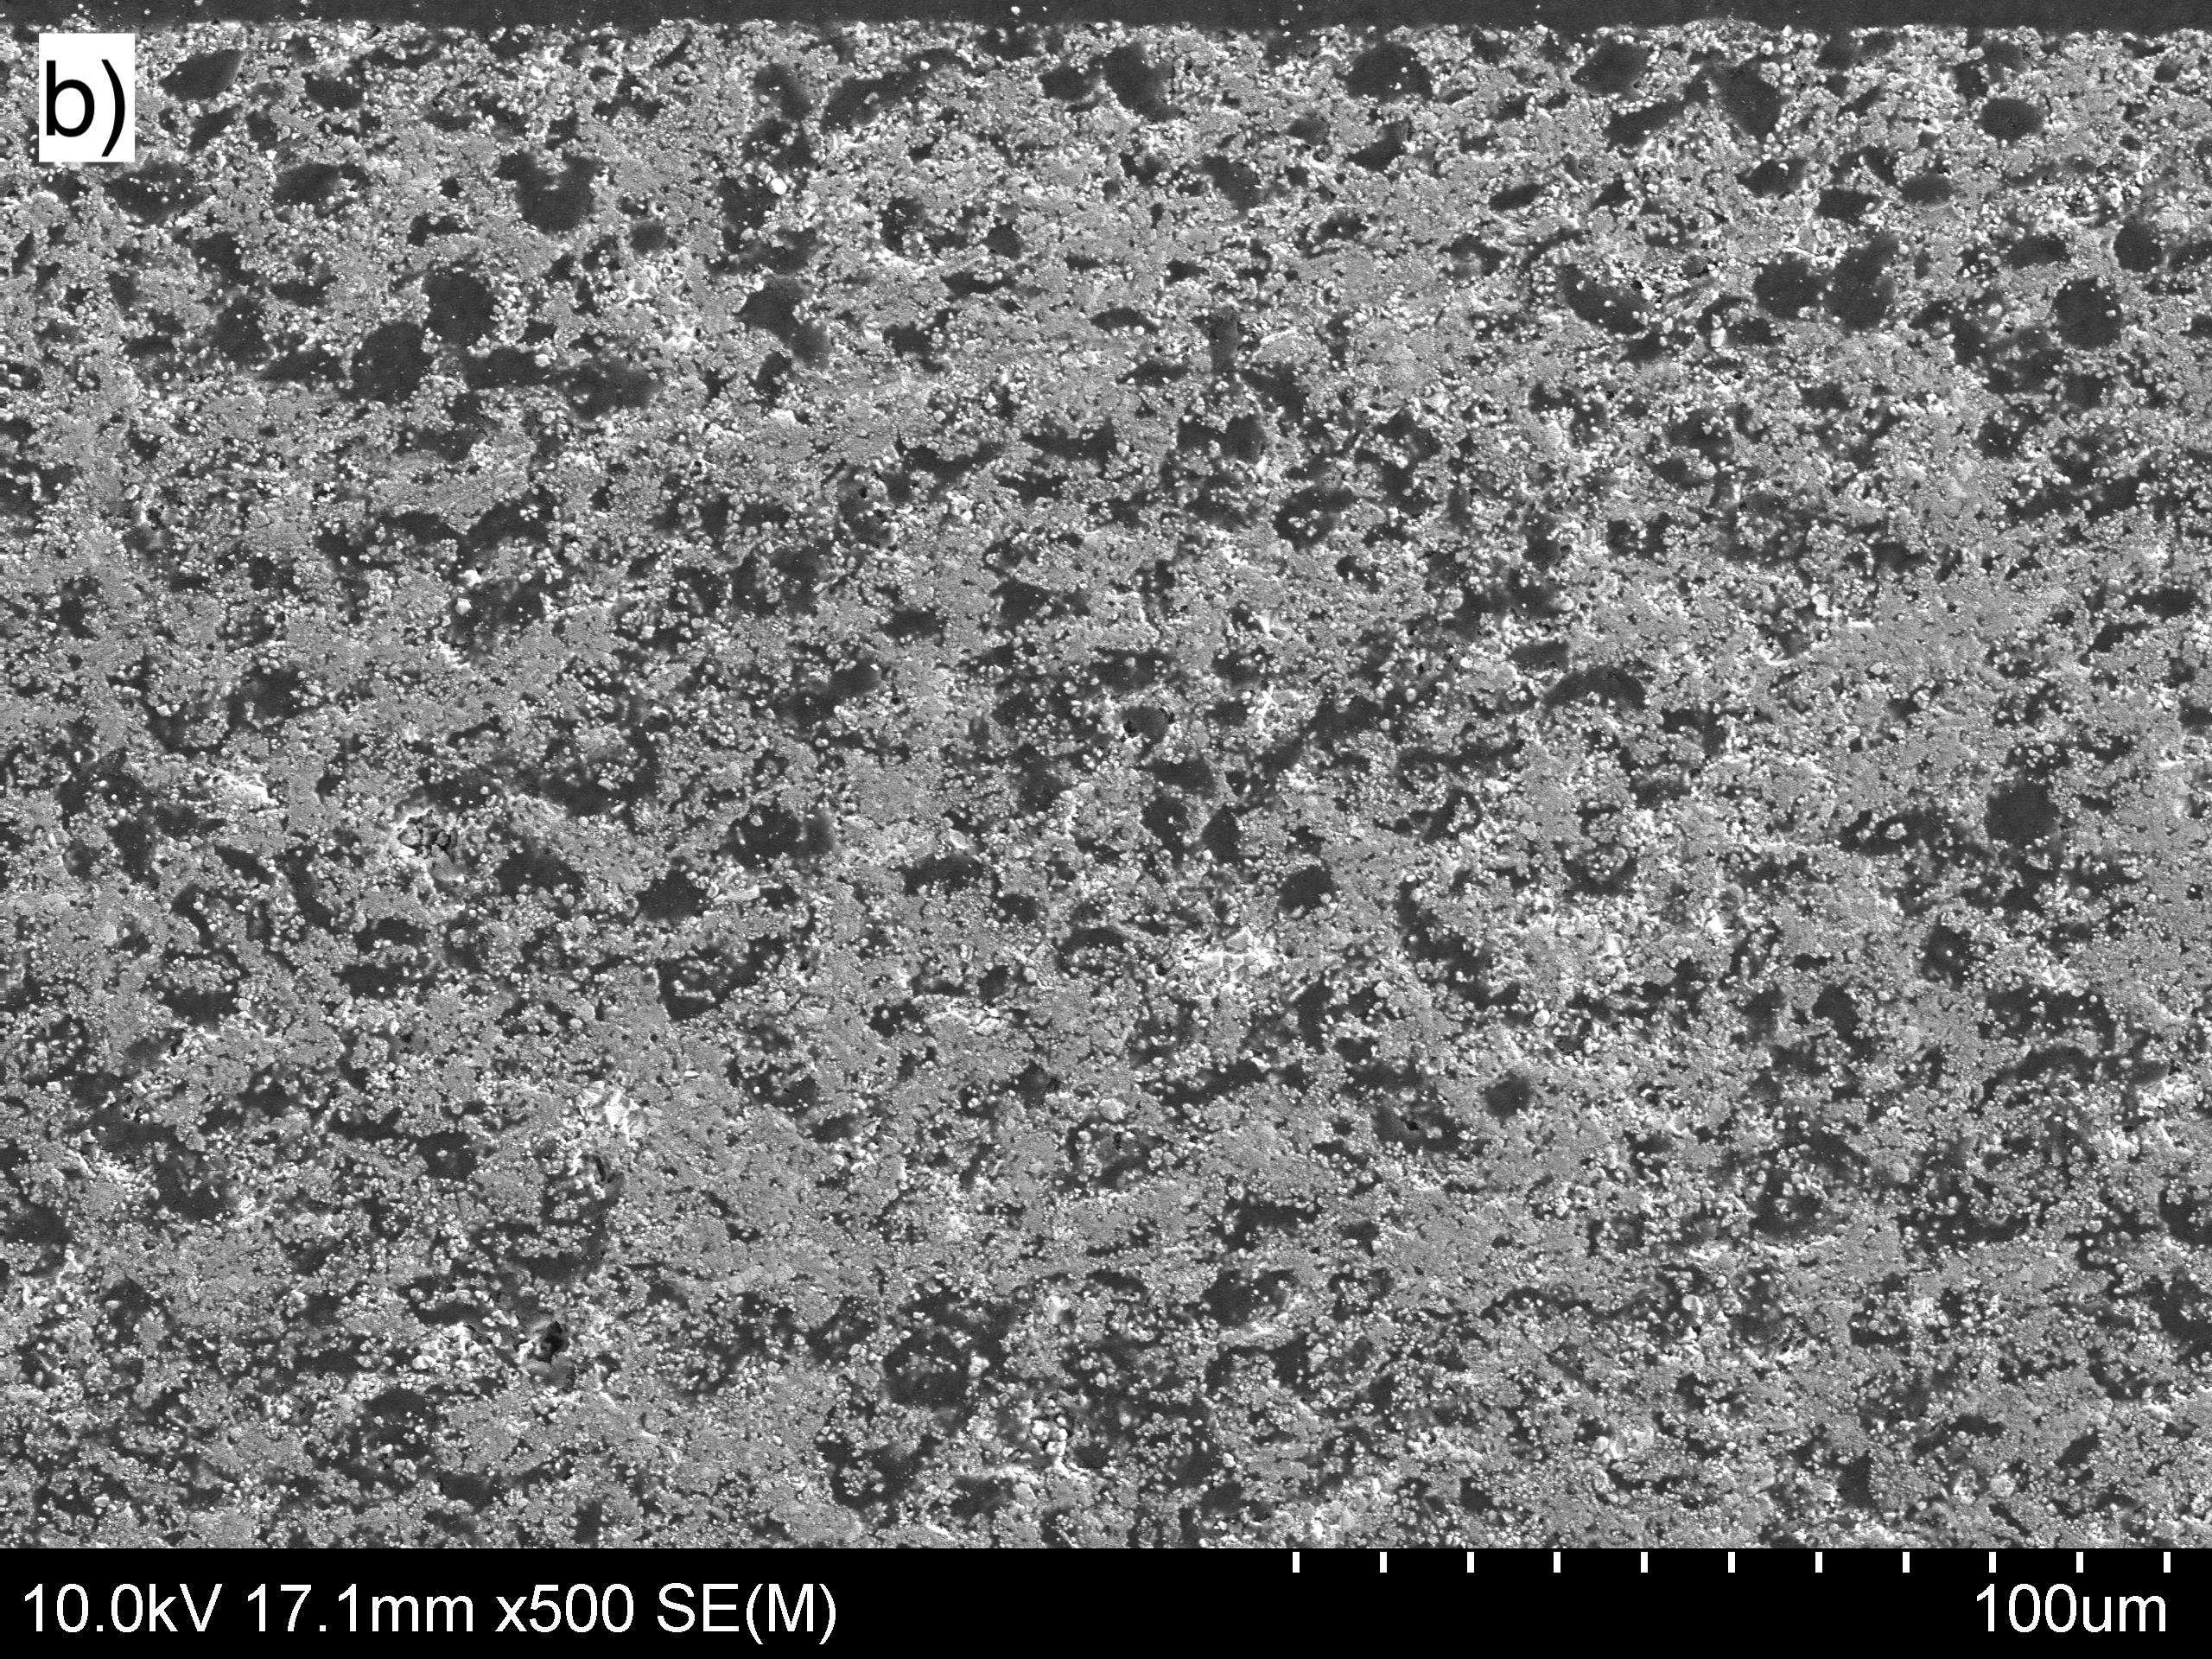
\includegraphics[width=0.45\textwidth]{10cycles.jpg}
          \caption{Scanning electron microscope images of epoxy filled and polished SFCM-GDC ASL  cross sections tested a) before any cycling, b) after 10 cycles between 10\% H\textsubscript{2} and N\textsubscript{2}.}
          \label{fig:cycledSEM}
        \end{figure}

\section{Conclusions}
    In this work the mechanical properties of SFCM and SFCM-GDC structures are characterized as the environment is changed from ambient to the working conditions of SOFCs and with redox cycling.
    The electrical conductivity of SFCM-GDC is stable up to 19 cycles due to the reversibility and phase stability of SFCM-GDC in the environment range.
    The fracture toughness of SFCM was found to be \SI[separate-uncertainty = true]{0.124 +- 0.023}{\mega\pascal\sqrt{m}} at room temperature and increases with temperature, due to relaxation of residual stresses.
    The flexural strength of SFCM-GDC/GDC half-cells increases by 23.9\% upon heating from room temperature to \SI{600}{\celsius}.
    This is due to thermal expansion pushing cracks closed during heating, requiring additional stress to propagate surface cracks and the increase in fracture toughness.
    Once exposed to reducing conditions, the flexural strength decreases by 29.4\% of the original strength, as SFCM and GDC generate oxygen vacancies.
    Reduction was shown to increase the size and variability of the distribution of flaws which lead to failure.
    Redox cycling led to the uniform increase in critical flaw size and changed the fine microstructural porosity, decreasing strength from \SI{34.3}{\mega\pascal} to \SI{22.4}{\mega\pascal}.

    These findings show that SFCM, when combined with GDC, make a suitable anode material for SOFCs.
    SFCM-GDC is a stable material system, both in terms of conductivity and mechanically, with redox cycling.
    Reduction does increase the likelihood of failure by decreasing characteristic strength and the distribution of flaws, but repeated cycling only decreases characteristic strength and does not change the Weibull modulus.
